% !TeX program = xelatex
\documentclass[a4paper,10pt]{article}

% ============================================================================
% ១. កញ្ចប់បណ្ណាល័យ និងការកំណត់ទំព័រ (Packages & Page Setup — តាមគំរូ ls_plan.tex)
% ============================================================================
\usepackage[a4paper, left=0.95cm, right=0.95cm, top=0.85cm, bottom=0.92cm, footskip=0.52cm]{geometry}
\usepackage{amsmath}
\usepackage{unicode-math}
\usepackage{fontspec}
\usepackage{longtable, array, multirow, colortbl}
\usepackage[table]{xcolor}
\usepackage{enumitem}
\usepackage{pifont}
\usepackage{fancyhdr}
\usepackage{tikz}
\usetikzlibrary{calc, arrows.meta, decorations.pathreplacing, patterns, positioning, babel}

\makeatletter
\let\@expl@@@mark@update@singlecol@structures@@\relax
\makeatother

% --- ប្រព័ន្ធស្វែងរកទីតាំងពុម្ពអក្សរស្វ័យប្រវត្តិ (Windows Local + Cloud Repo fonts/) ---
\providecommand{\NGSFindFonts}{%
  \IfFileExists{C:/Windows/Fonts/cambria.ttc}{%
    \def\NGSSysPath{C:/Windows/Fonts/}%
    \def\NGSUserPath{C:/Users/KIT/AppData/Local/Microsoft/Windows/Fonts/}%
  }{%
    \IfFileExists{./fonts/KhmerOSsiemreap.ttf}{\def\NGSSysPath{./fonts/}\def\NGSUserPath{./fonts/}}{%
    \IfFileExists{../fonts/KhmerOSsiemreap.ttf}{\def\NGSSysPath{../fonts/}\def\NGSUserPath{../fonts/}}{%
    \IfFileExists{../../fonts/KhmerOSsiemreap.ttf}{\def\NGSSysPath{../../fonts/}\def\NGSUserPath{../../fonts/}}{%
    \IfFileExists{../../../fonts/KhmerOSsiemreap.ttf}{\def\NGSSysPath{../../../fonts/}\def\NGSUserPath{../../../fonts/}}{%
    \IfFileExists{../../../../fonts/KhmerOSsiemreap.ttf}{\def\NGSSysPath{../../../../fonts/}\def\NGSUserPath{../../../../fonts/}}{%
    \IfFileExists{../../../../../fonts/KhmerOSsiemreap.ttf}{\def\NGSSysPath{../../../../../fonts/}\def\NGSUserPath{../../../../../fonts/}}{%
    \IfFileExists{../../../../../../fonts/KhmerOSsiemreap.ttf}{\def\NGSSysPath{../../../../../../fonts/}\def\NGSUserPath{../../../../../../fonts/}}{%
      \def\NGSSysPath{../../../../../../../fonts/}\def\NGSUserPath{../../../../../../../fonts/}%
    }}}}}}}%
  }%
}
\NGSFindFonts

% ============================================================================
% ២. កំណត់ពុម្ពអក្សរ (Fonts — តាមគំរូ ls_plan.tex)
% ============================================================================
\setmathfont[Path={\NGSSysPath}, FontIndex=1, Scale=1.02]{cambria.ttc}
\defaultfontfeatures{Ligatures=TeX}

\setmainfont[
  Path={\NGSUserPath},
  Extension=.ttf,
  Script=Khmer,
  BoldFont={KhmerOSsiemreap},
  BoldFeatures={FakeBold=1.8},
  ItalicFont={KhmerOSsiemreap},
  ItalicFeatures={FakeSlant=0.25},
  BoldItalicFont={KhmerOSsiemreap},
  BoldItalicFeatures={FakeBold=1.8, FakeSlant=0.25}
]{KhmerOSsiemreap}

\newfontfamily\muol[Path={\NGSUserPath}, Extension=.ttf, Script=Khmer]{KhmerOSmuollight}
\newfontfamily\Tacteing[Path={\NGSUserPath}, Extension=.TTF]{TACTENG}
\newfontfamily\TimesEn[Path={\NGSSysPath}, Extension=.ttf, BoldFont={timesbd}, ItalicFont={timesi}, BoldItalicFont={timesbi}]{times}
\newfontfamily\CalibriFont[Path={\NGSSysPath}, Extension=.ttf]{calibri}
\newfontfamily\CourierCirc[Path={\NGSSysPath}, Extension=.ttf]{cour}

\XeTeXlinebreaklocale "km"
\XeTeXlinebreakskip = 0pt plus 1pt minus 0.1pt

% ============================================================================
% ៣. ពណ៌ និងការតុបតែង (Colors & Styles)
% ============================================================================
\definecolor{stepbg}{HTML}{D9D9D9}
\definecolor{headgray}{HTML}{E6E6E6}
\definecolor{emphred}{HTML}{C00000}

\pagestyle{fancy}
\fancyhf{}
\renewcommand{\headrulewidth}{0pt}
\fancyfoot[R]{\CalibriFont\fontsize{9pt}{11pt}\selectfont\thepage}

\setlength{\parindent}{0pt}
\setlength{\parskip}{0pt}
\setlength{\tabcolsep}{4.5pt}
\setlength{\LTpre}{2pt}
\setlength{\LTpost}{2pt}

\newcolumntype{L}[1]{>{\raggedright\arraybackslash}p{#1}}
\newcolumntype{C}[1]{>{\centering\arraybackslash}p{#1}}

% ============================================================================
% ៤. ពាក្យបញ្ជាជំនួយ (Helper Macros)
% ============================================================================
\newcommand{\en}[1]{{\TimesEn #1}}
\newcommand{\enbf}[1]{{\TimesEn\bfseries #1}}
\newcommand{\khmflourish}{{\Tacteing\fontsize{15pt}{15pt}\selectfont 3}}
\newcommand{\wcirc}{{\CourierCirc\fontsize{9.5pt}{11pt}\selectfont o}}
\newcommand{\ditem}{{\fontsize{7.5pt}{10pt}\selectfont\ding{117}}\ }
\newcommand{\fiveE}[1]{\textcolor{emphred}{\CalibriFont\bfseries #1}}
\newcommand{\redsub}[1]{\textcolor{emphred}{#1}}
\newcommand{\timenote}[1]{\textcolor{emphred}{\textit{#1}}}
\newcommand{\stepheader}[1]{\multicolumn{3}{|c|}{\cellcolor{stepbg}\muol #1} \\ \hline}
\newcommand{\cfig}[1]{{\centering\vspace{3pt}#1\vspace{3pt}\par}}
\newcommand{\cnum}[1]{\mbox{\fontsize{10.5pt}{12pt}\selectfont\ding{\numexpr181+#1\relax}}}
\newcommand{\unit}[1]{\,\text{\en{#1}}}
\newcommand{\riel}{\,\text{៛}}
\newcommand{\graybox}[1]{\colorbox{headgray}{\strut #1}}

% ============================================================================
% ៥. រូបភាព TikZ ស-ខ្មៅ សម្រាប់បង្រៀនលើក្ដារខៀន និងសន្លឹកកិច្ចការ (B&W Diagrams)
% ============================================================================

% ១. E1 Engage: អន្ទាក់សម្រួលមុនប្ដូរសញ្ញាចែកក្នុង (a^2-9)/(3a) ÷ (a+3)/(a-3) (ទំ.៨០)
\newcommand{\figEngageRATSixThree}{%
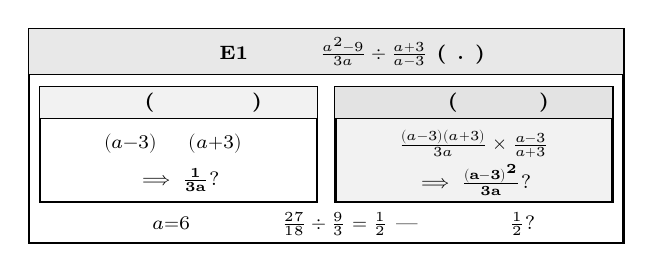
\begin{tikzpicture}[x=1cm, y=1cm, every node/.style={font=\scriptsize, text=black}]
  \draw[black, line width=0.9pt] (0,0) rectangle (7.55,2.72);
  \fill[gray!18] (0,2.14) rectangle (7.55,2.72);
  \draw[black, line width=0.6pt] (0,2.14) -- (7.55,2.14);
  \node at (3.775,2.43) {\textbf{បេសកកម្ម \en{E1}៖ គណនាផលចែក $\tfrac{a^2 - 9}{3a} \div \tfrac{a + 3}{a - 3}$ (ទំ.៨០)}};

  % Student A
  \draw[black, line width=0.8pt] (0.14,0.52) rectangle (3.66,1.98);
  \fill[gray!10] (0.14,1.58) rectangle (3.66,1.98);
  \draw[black, line width=0.5pt] (0.14,1.58) -- (3.66,1.58);
  \node at (1.90,1.78) {\textbf{សិស្ស ក (សម្រួលឆ្លងសញ្ញាចែក)}};
  \node at (1.90,1.26) {ឈូត $(a{-}3)$ និង $(a{+}3)$ ភ្លាម};
  \node at (1.90,0.80) {$\implies \mathbf{\tfrac{1}{3a}}$?};

  % Student B
  \draw[black, line width=0.95pt, fill=gray!10] (3.89,0.52) rectangle (7.41,1.98);
  \fill[gray!22] (3.89,1.58) rectangle (7.41,1.98);
  \draw[black, line width=0.55pt] (3.89,1.58) -- (7.41,1.58);
  \node at (5.65,1.78) {\textbf{សិស្ស ខ (គុណនឹងចម្រាសសិន)}};
  \node at (5.65,1.26) {$\tfrac{(a-3)(a+3)}{3a} \times \tfrac{a-3}{a+3}$};
  \node at (5.65,0.80) {$\implies \mathbf{\tfrac{(a - 3)^2}{3a}}$?};

  \node at (3.775,0.24) {\textbf{តេស្ត $a{=}6$៖} កន្សោមដើមស្មើ $\tfrac{27}{18} \div \tfrac{9}{3} = \tfrac{1}{2}$ — តើចម្លើយណាស្មើ $\tfrac{1}{2}$?};
\end{tikzpicture}}

% ២. E2 Explore: វិធីគុណ (ទំ.៧៨--៧៩) និងវិធីចែក (ទំ.៧៩--៨០)
\newcommand{\figExploreRATSixThree}{%
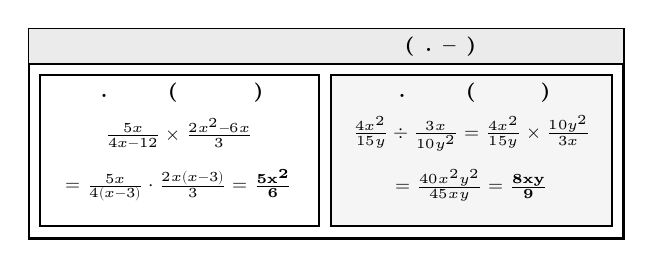
\begin{tikzpicture}[x=1cm, y=1cm, every node/.style={font=\scriptsize, text=black}]
  \draw[black, line width=0.9pt] (0,0) rectangle (7.55,2.66);
  \fill[gray!16] (0,2.22) rectangle (7.55,2.66);
  \draw[black, line width=0.6pt] (0,2.22) -- (7.55,2.22);
  \node at (3.775,2.44) {\textbf{ប្រៀបធៀបជំហានគុណ និងជំហានចែកកន្សោមសនិទាន (ទំ.៧៨--៨០)}};

  % Left: Multiplication
  \draw[black, line width=0.8pt] (0.14,0.16) rectangle (3.68,2.08);
  \node at (1.91,1.86) {\textbf{៤.១ វិធីគុណ (ដាក់ជាកត្តាសិន)}};
  \node at (1.91,1.34) {$\tfrac{5x}{4x-12} \times \tfrac{2x^2-6x}{3}$};
  \node at (1.91,0.68) {$= \tfrac{5x}{4(x-3)} \cdot \tfrac{2x(x-3)}{3} = \mathbf{\tfrac{5x^2}{6}}$};

  % Right: Division
  \draw[black, line width=0.8pt, fill=gray!8] (3.84,0.16) rectangle (7.41,2.08);
  \node at (5.625,1.86) {\textbf{៤.២ វិធីចែក (គុណនឹងចម្រាស)}};
  \node at (5.625,1.34) {$\tfrac{4x^2}{15y} \div \tfrac{3x}{10y^2} = \tfrac{4x^2}{15y} \times \tfrac{10y^2}{3x}$};
  \node at (5.625,0.68) {$= \tfrac{40x^2y^2}{45xy} = \mathbf{\tfrac{8xy}{9}}$};
\end{tikzpicture}}

% ៣. E3 Explain: រូបមន្តគុណ A/B × C/D និងចែក A/B ÷ C/D (ទំ.៧៩--៨០)
\newcommand{\figRuleRATSixThree}{%
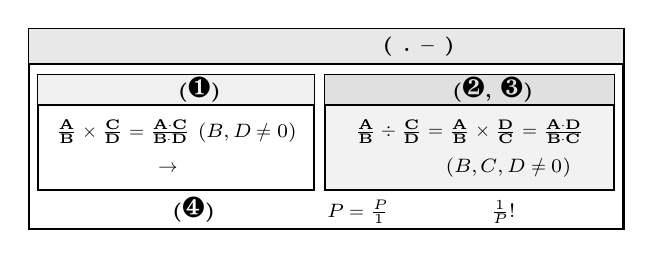
\begin{tikzpicture}[x=1cm, y=1cm, every node/.style={font=\scriptsize, text=black}]
  \draw[black, line width=0.9pt] (0,0) rectangle (7.55,2.54);
  \fill[gray!18] (0,2.10) rectangle (7.55,2.54);
  \draw[black, line width=0.6pt] (0,2.10) -- (7.55,2.10);
  \node at (3.775,2.32) {\textbf{វិធានគុណ និងវិធានចែកកន្សោមសនិទាន (ទំ.៧៩--៨០)}};

  % Left: Multiplication Rule
  \draw[black, line width=0.8pt] (0.12,0.50) rectangle (3.62,1.96);
  \fill[gray!12] (0.12,1.58) rectangle (3.62,1.96);
  \draw[black, line width=0.55pt] (0.12,1.58) -- (3.62,1.58);
  \node at (1.87,1.77) {\textbf{វិធីគុណ (\cnum{1})}};
  \node at (1.87,1.24) {$\mathbf{\tfrac{A}{B} \times \tfrac{C}{D} = \tfrac{A \cdot C}{B \cdot D}}$ ($B, D \neq 0$)};
  \node at (1.87,0.78) {ដាក់ជាកត្តា $\to$ សម្រួលកត្តារួម};

  % Right: Division Rule
  \draw[black, line width=0.95pt, fill=gray!10] (3.76,0.50) rectangle (7.43,1.96);
  \fill[gray!24] (3.76,1.58) rectangle (7.43,1.96);
  \draw[black, line width=0.6pt] (3.76,1.58) -- (7.43,1.58);
  \node at (5.595,1.77) {\textbf{វិធីចែក (\cnum{2}, \cnum{3})}};
  \node at (5.595,1.24) {$\mathbf{\tfrac{A}{B} \div \tfrac{C}{D} = \tfrac{A}{B} \times \tfrac{D}{C} = \tfrac{A \cdot D}{B \cdot C}}$};
  \node at (5.595,0.78) {ត្រឡប់តែតួចែក ($B, C, D \neq 0$)};

  \node at (3.775,0.24) {\textbf{ចំណាំ (\cnum{4})៖} កន្សោមគ្មានភាគបែង $P = \tfrac{P}{1}$ មានចម្រាសស្មើនឹង $\tfrac{1}{P}$!};
\end{tikzpicture}}

% ៤. E4 Elaborate: លំហាត់គំរូវិធីគុណ (ទំ.៧៩) និងវិធីចែក (ទំ.៨០)
\newcommand{\figElaborateRATSixThree}{%
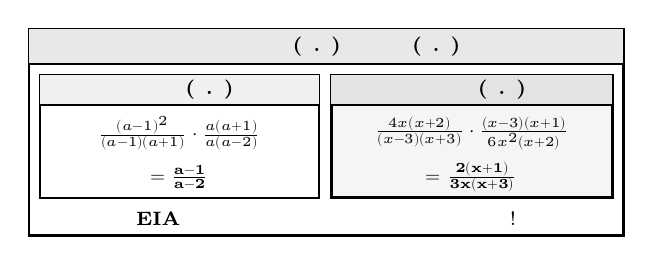
\begin{tikzpicture}[x=1cm, y=1cm, every node/.style={font=\scriptsize, text=black}]
  \draw[black, line width=0.9pt] (0,0) rectangle (7.55,2.62);
  \fill[gray!18] (0,2.18) rectangle (7.55,2.62);
  \draw[black, line width=0.6pt] (0,2.18) -- (7.55,2.18);
  \node at (3.775,2.40) {\textbf{លំហាត់គំរូវិធីគុណ (ទំ.៧៩) និងវិធីចែក (ទំ.៨០)}};

  % Left: Mult Worked Example
  \draw[black, line width=0.8pt] (0.14,0.48) rectangle (3.68,2.04);
  \fill[gray!12] (0.14,1.66) rectangle (3.68,2.04);
  \draw[black, line width=0.55pt] (0.14,1.66) -- (3.68,1.66);
  \node at (1.91,1.85) {\textbf{គំរូគុណ ក (ទំ.៧៩)}};
  \node at (1.91,1.30) {$\tfrac{(a-1)^2}{(a-1)(a+1)} \cdot \tfrac{a(a+1)}{a(a-2)}$};
  \node at (1.91,0.74) {$= \mathbf{\tfrac{a - 1}{a - 2}}$};

  % Right: Div Worked Example
  \draw[black, line width=0.95pt, fill=gray!8] (3.84,0.48) rectangle (7.41,2.04);
  \fill[gray!22] (3.84,1.66) rectangle (7.41,2.04);
  \draw[black, line width=0.6pt] (3.84,1.66) -- (7.41,1.66);
  \node at (5.625,1.85) {\textbf{គំរូចែក ខ (ទំ.៨០)}};
  \node at (5.625,1.30) {$\tfrac{4x(x+2)}{(x-3)(x+3)} \cdot \tfrac{(x-3)(x+1)}{6x^2(x+2)}$};
  \node at (5.625,0.74) {$= \mathbf{\tfrac{2(x + 1)}{3x(x + 3)}}$};

  \node at (3.775,0.22) {\textbf{\en{EIA}៖} ការដាក់ជាផលគុណកត្តាមុនគុណពង្រីក ជួយឱ្យសម្រួលកត្តារួមភ្លាមៗ!};
\end{tikzpicture}}

% ៥. E5 Evaluate: ជម្រើសវិនិច្ឆ័យ A-D សម្រាប់ 2x/(x-1) ÷ 4x^2/(x-1)
\newcommand{\figExitRATSixThree}{%
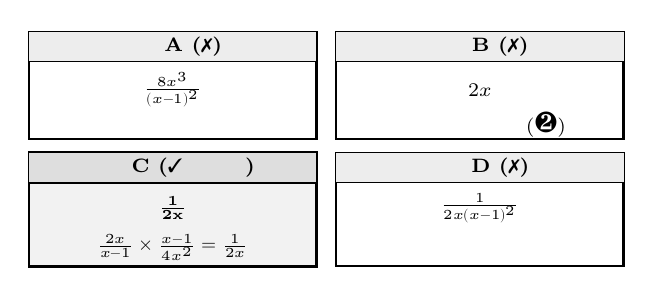
\begin{tikzpicture}[x=1cm, y=1cm, every node/.style={font=\scriptsize, text=black}]
  % Choice A
  \draw[black, line width=0.8pt] (0,1.62) rectangle (3.65,2.98);
  \fill[gray!14] (0,2.60) rectangle (3.65,2.98);
  \draw[black, line width=0.5pt] (0,2.60) -- (3.65,2.60);
  \node at (1.825,2.79) {\textbf{ជម្រើស \en{A} (\ding{55})}};
  \node at (1.825,2.24) {$\tfrac{8x^3}{(x - 1)^2}$};
  \node at (1.825,1.80) {គុណត្រង់ៗ ភ្លេចត្រឡប់តួចែក};

  % Choice B
  \draw[black, line width=0.8pt] (3.90,1.62) rectangle (7.55,2.98);
  \fill[gray!14] (3.90,2.60) rectangle (7.55,2.98);
  \draw[black, line width=0.5pt] (3.90,2.60) -- (7.55,2.60);
  \node at (5.725,2.79) {\textbf{ជម្រើស \en{B} (\ding{55})}};
  \node at (5.725,2.24) {$2x$};
  \node at (5.725,1.80) {ត្រឡប់ខុសប្រភាគតំណាងចែក (\cnum{2})};

  % Choice C (Correct)
  \draw[black, line width=1.0pt, fill=gray!10] (0,0) rectangle (3.65,1.44);
  \fill[gray!26] (0,1.06) rectangle (3.65,1.44);
  \draw[black, line width=0.55pt] (0,1.06) -- (3.65,1.06);
  \node at (1.825,1.25) {\textbf{ជម្រើស \en{C} (\ding{51} ត្រឹមត្រូវ)}};
  \node at (1.825,0.74) {$\mathbf{\tfrac{1}{2x}}$};
  \node at (1.825,0.24) {$\tfrac{2x}{x-1} \times \tfrac{x-1}{4x^2} = \tfrac{1}{2x}$};

  % Choice D
  \draw[black, line width=0.8pt] (3.90,0) rectangle (7.55,1.44);
  \fill[gray!14] (3.90,1.06) rectangle (7.55,1.44);
  \draw[black, line width=0.5pt] (3.90,1.06) -- (7.55,1.06);
  \node at (5.725,1.25) {\textbf{ជម្រើស \en{D} (\ding{55})}};
  \node at (5.725,0.74) {$\tfrac{1}{2x(x - 1)^2}$};
  \node at (5.725,0.24) {ត្រឡប់តួចែក តែភ្លេចសម្រួល};
\end{tikzpicture}}

% ============================================================================
% ៦. ចាប់ផ្ដើមឯកសារ (Document Body)
% ============================================================================
\begin{document}
\fontsize{10pt}{15.2pt}\selectfont

% --- ក្បាលរដ្ឋបាល (Administrative Header) ---
\begin{center}
  {\muol\fontsize{11pt}{16pt}\selectfont ព្រះរាជាណាចក្រកម្ពុជា}\\[2pt]
  {\muol\fontsize{11pt}{16pt}\selectfont ជាតិ សាសនា ព្រះមហាក្សត្រ}\\[-2pt]
  \khmflourish
\end{center}
\vspace{-4pt}

{\muol\fontsize{10pt}{15pt}\selectfont
មន្ទីរអប់រំ យុវជន និងកីឡា ខេត្តកំពង់ធំ\\
ការិយាល័យអប់រំ យុវជន និងកីឡា ស្រុកកំពង់ស្វាយ\\
អនុវិទ្យាល័យព្រះក្រសាំង}

\vspace{2pt}
\begin{center}
  {\muol\fontsize{12pt}{18pt}\selectfont កិច្ចតែងការបង្រៀន}
\end{center}
\vspace{1pt}

% --- ព័ត៌មានទូទៅ (General Metadata) ---
\begin{tabular}{@{}p{1.85cm}p{3.25cm}@{\hspace{4pt}:\hspace{6pt}}p{12.65cm}@{}}
  & - \quad មុខវិជ្ជា          & គណិតវិទ្យា ថ្នាក់ទី៨ (ពីជគណិត) \\
  & - \quad ចំណងជើងមេរៀន & មេរៀនទី៦៖ កន្សោមសនិទាន \\
  & - \quad ចំណងជើងរង      & ៤. វិធីគុណនិងវិធីចែកកន្សោមសនិទាន \\
  & - \quad រយៈពេល             & ១ ម៉ោងសិក្សា (៥០ នាទី) \\
  & - \quad បង្រៀនដោយ         & ហុក ប៊ុនថែន \\
  & - \quad កាលបរិច្ឆេទ        & ថ្ងៃពុធ ទី១៦ ខែធ្នូ ឆ្នាំ២០២៦ \\
\end{tabular}

\vspace{4pt}

% --- I. វត្ថុបំណង ---
{\muol\enbf{I.} វត្ថុបំណង}\par\vspace{2pt}
\begin{tabular}{@{}p{0.55cm}p{2.55cm}@{\hspace{2pt}:\hspace{6pt}}L{15.4cm}@{}}
  & \wcirc វិជ្ជាសម្បទា   & សិស្សប្រាប់បាននូវវិធានគុណ $\tfrac{A}{B}\times\tfrac{C}{D} = \tfrac{AC}{BD}$ និងវិធានចែកកន្សោមសនិទាន $\tfrac{A}{B}\div\tfrac{C}{D} = \tfrac{A}{B}\times\tfrac{D}{C} = \tfrac{AD}{BC}$ បានត្រឹមត្រូវ (ទំ.៧៨–៨០) ។ \\[2pt]
  & \wcirc បំណិនសម្បទា & សិស្សដាក់ជាផលគុណកត្តា និងគណនាផលគុណព្រមទាំងផលចែកនៃកន្សោមសនិទានលើសន្លឹកកិច្ចការបានត្រឹមត្រូវ ។ \\[2pt]
  & \wcirc ចរិយាសម្បទា  & សិស្សមានទម្លាប់ប្ដូរសញ្ញាចែកជាគុណនឹងចម្រាសនៃប្រភាគតួចែកជាមុនសិនមុននឹងសម្រួលកត្តារួមប្រកបដោយភាពម៉ត់ចត់ ។ \\
\end{tabular}

\vspace{3pt}

% --- II. សម្ភារៈឧបទេស (Zero-LCD & Fill-In Worksheet Context) ---
{\muol\enbf{II.} សម្ភារៈឧបទេស}\par\vspace{2pt}
\hspace*{0.55cm}$\bullet$ សៀវភៅសិក្សាគោលថ្នាក់ទី៨ (ទំ.៧៨--៨០, ៨៦) ក្ដារខៀន ដីស/ហ្វឺត បន្ទាត់ត្រង់ និង\textbf{សន្លឹកកិច្ចការសិស្សបំពេញចន្លោះ ស-ខ្មៅ} (កូដ \en{RAT63} ទំព័រ ១--២ សម្រាប់សិស្ស និងទំព័រ ៣ ប្លង់ក្ដារខៀន/ចម្លើយគ្រូ — គ្មានប្រើ \en{LCD})

\vspace{3pt}

% --- III. វិធីសាស្រ្តបង្រៀន ---
{\muol\enbf{III.} វិធីសាស្រ្តបង្រៀន}\par\vspace{2pt}
\begin{tabular}{@{}p{0.55cm}p{2.55cm}@{\hspace{2pt}:\hspace{6pt}}L{15.4cm}@{}}
  & $\bullet$ គោលវិធី      & សិស្សមជ្ឈមណ្ឌល (សន្លឹកកិច្ចការបំពេញចន្លោះជាគោល + ការពិភាក្សាជាក្រុមតូច ៣ នាក់) \\
  & $\bullet$ យុទ្ធវិធីបង្រៀន & គំរូស្ថាបនានិយម \en{5Es} រួមបញ្ចូល \textit{ការវិភាគលំហាត់គំរូខុស (\en{Erroneous Examples})} និង \textit{ការប្រៀបធៀបគុណ-ចែក} \\
\end{tabular}

\vspace{4pt}

% --- IV. ដំណើរការបង្រៀន (50-Minute 5E Flow) ---
{\muol\enbf{IV.} ដំណើរការបង្រៀន}\par\vspace{1pt}

\renewcommand{\arraystretch}{1.15}
\begin{longtable}{|L{5.50cm}|L{7.90cm}|L{4.80cm}|}
\hline
\multicolumn{1}{|c|}{\cellcolor{headgray}\muol សកម្មភាពគ្រូ} &
\multicolumn{1}{c|}{\cellcolor{headgray}\muol ខ្លឹមសារមេរៀន} &
\multicolumn{1}{c|}{\cellcolor{headgray}\muol សកម្មភាពសិស្ស} \\[2pt]
\hline
\endfirsthead

\hline
\multicolumn{1}{|c|}{\cellcolor{headgray}\muol សកម្មភាពគ្រូ} &
\multicolumn{1}{c|}{\cellcolor{headgray}\muol ខ្លឹមសារមេរៀន} &
\multicolumn{1}{c|}{\cellcolor{headgray}\muol សកម្មភាពសិស្ស} \\[2pt]
\hline
\endhead

\hline
\endfoot

% ==================== ជំហានទី១ (2min) ====================
\stepheader{ជំហានទី១ \enbf{(}រដ្ឋបាលថ្នាក់\enbf{)}}
$\bullet$ ពិនិត្យវត្តមាន អនាម័យ និងសណ្ដាប់ធ្នាប់ថ្នាក់រៀន \par
$\bullet$ រៀបចំក្រុមតូច ៣ នាក់ និងចែក\textbf{សន្លឹកកិច្ចការសិស្ស} (\en{RAT63} ទំព័រ ១–២)
&
$\bullet$ រដ្ឋបាលថ្នាក់ អនាម័យ និងវិន័យសិក្សា \par
$\bullet$ ចែកសន្លឹកកិច្ចការម្នាក់ ១ សន្លឹក សម្រាប់បំពេញតាមដំណាក់កាល \en{E1--E5}
&
$\circ$ ប្រធានថ្នាក់រាយការណ៍វត្តមានសិស្ស \par
$\circ$ ទទួលសន្លឹកកិច្ចការ សរសេរឈ្មោះ និងអង្គុយតាមក្រុម ៣ នាក់ \\
\hline

% ==================== ជំហានទី២ (9min: កំណែ ≤3m + រំលឹក 3m + E1 3m) ====================
\stepheader{ជំហានទី២ \enbf{(}កិច្ចការផ្ទះ \enbf{+} ទំនាក់ទំនងមេរៀនថ្មី\enbf{)}}
\ditem \textbf{កំណែកិច្ចការផ្ទះ (\enbf{$\le$ 3 min})} \par
$\bullet$ ហៅសិស្ស ២ នាក់ឡើងកែលំហាត់ទំ.៨៥ \en{\#5} ខ, គ និង \en{\#5} ដ, ឍ លើក្ដារខៀន
&
\hspace*{0.15cm}\redsub{កំណែកិច្ចការផ្ទះ (ទំ.៨៥ លេខ ៥ ខ, គ, ដ, ឋ, ឍ)} \par
$\bullet$ \textbf{\en{\#5} ខ, គ៖} ខ) $\tfrac{-8a^2b^4x}{-8a^3b^3x^3} = \mathbf{\tfrac{b}{ax^2}}$; \quad គ) $\tfrac{x(a-b)^2}{(a-b)^3} = \mathbf{\tfrac{x}{a - b}}$ \par
$\bullet$ \textbf{\en{\#5} ដ, ឋ, ឍ៖} ដ) $\mathbf{\tfrac{a - b}{a + b}}$; \quad ឋ) $\mathbf{\tfrac{a - 1}{3}}$; \quad ឍ) $\mathbf{\tfrac{a + 6}{a + 4}}$
&
$\circ$ ផ្ទៀងចម្លើយ និងកែតម្រូវចូលសៀវភៅកិច្ចការផ្ទះ \\[3pt]

\ditem \textbf{រំលឹកមេរៀនទាក់ទង (\enbf{3min})} \par
$\bullet$ សួរ៖ «តើគេគុណប្រភាគ $\tfrac{4}{9} \times \tfrac{3}{8}$ និងចែកប្រភាគ $\tfrac{3}{2} \div \tfrac{2}{5}$ (ទំ.៧៨–៧៩) ដោយវិធីណា?»
&
\hspace*{0.15cm}\redsub{រំលឹកវិធីគុណ និងវិធីចែកប្រភាគចំនួនសនិទាន (ទំ.៧៨–៧៩)} \par
$\bullet$ វិធីគុណ៖ $\tfrac{4}{9} \times \tfrac{3}{8} = \tfrac{4 \times 3}{9 \times 8} = \tfrac{1}{6}$ (សម្រួលកត្តារួមមុនគុណកាន់តែលឿន) \par
$\bullet$ វិធីចែក៖ $\tfrac{3}{2} \div \tfrac{2}{5} = \tfrac{3}{2} \times \tfrac{5}{2} = \tfrac{15}{4}$ (គុណនឹងចម្រាសនៃប្រភាគតួចែក)
&
$\circ$ ឆ្លើយ៖ «គុណភាគយកនឹងភាគយក ឯវិធីចែកគុណនឹងចម្រាសនៃតួចែក!» \\[3pt]

\fiveE{E1 - Engage (3min)} \timenote{(កុំទាន់ផ្តល់ចម្លើយ)} \par
\ditem \textbf{បេសកកម្មអន្ទាក់សម្រួលមុនប្ដូរសញ្ញាចែក (សន្លឹកកិច្ចការ \en{E1})} \par
$\bullet$ ឱ្យសិស្សអានប្រអប់ \en{E1} ពិនិត្យផលចែក $\dfrac{a^2 - 9}{3a} \div \dfrac{a + 3}{a - 3}$ (ទំ.៨០) ដោយជំនួស $a = 6$
&
\redsub{បេសកកម្ម \en{E1}៖ គណនា $\dfrac{a^2 - 9}{3a} \div \dfrac{a + 3}{a - 3}$ តាមវិធីណាទើបត្រូវ? (ទំ.៨០)} \par
$\bullet$ \textbf{សិស្ស ក} ឈូត $(a-3)$ និង $(a+3)$ ឆ្លងសញ្ញាចែកភ្លាម បាន $\dfrac{1}{3a}$! \par
$\bullet$ \textbf{សិស្ស ខ} ប្ដូរចែកជាគុណនឹងចម្រាសសិន បាន $\dfrac{(a - 3)^2}{3a}$! តេស្ត $a = 6$ មើល៍!
&
$\circ$ ជំនួស $a = 6$ ពិភាក្សាជាគូ និងគូស \ding{51} ក្នុងប្រអប់ \en{E1} \\[3pt]

&
\cfig{\figEngageRATSixThree}
& \\
\hline

% ==================== ជំហានទី៣ (17min: E2 11m + E3 6m) ====================
\stepheader{ជំហានទី៣ \enbf{(}ខ្លឹមសារមេរៀនថ្មី\enbf{)}}
\fiveE{E2 - Explore (11min)} \par
$\bullet$ សរសេរចំណងជើងរង \textbf{៤. វិធីគុណនិងវិធីចែកកន្សោមសនិទាន} លើក្ដារខៀន \par
\ditem \textbf{សកម្មភាព ១៖ ៤.១ វិធីគុណកន្សោមសនិទាន (ទំ.៧៨–៧៩, \enbf{5min}, \en{E2-A})} \par
$\bullet$ ឱ្យសិស្សបំពេញឧទាហរណ៍ទី ១ និងទី ២ នៃវិធីគុណលើ \en{E2-A}
&
៤.១ វិធីគុណកន្សោមសនិទាន (ទំ.៧៨–៧៩) \par
$\bullet$ \textbf{ឧទាហរណ៍ទី ១៖} $\dfrac{7b}{10a} \times \dfrac{5a^2}{8b} = \dfrac{35a^2b}{80ab} = \mathbf{\dfrac{7a}{16}}$ \par
$\bullet$ \textbf{ឧទាហរណ៍ទី ២៖} $\dfrac{5x}{4x - 12} \times \dfrac{2x^2 - 6x}{3} = \dfrac{5x}{4(x - 3)} \times \dfrac{2x(x - 3)}{3} = \mathbf{\dfrac{5x^2}{6}}$
&
$\circ$ ដាក់ជាផលគុណកត្តា និងគណនាផលគុណលើ \en{E2-A} \\[3pt]

\ditem \textbf{សកម្មភាព ២៖ ៤.២ វិធីចែកកន្សោមសនិទាន (ទំ.៧៩–៨០, \enbf{6min}, \en{E2-B})} \par
$\bullet$ ឱ្យសិស្សបំពេញឧទាហរណ៍ ក និង ខ នៃវិធីចែកដោយគុណនឹងចម្រាសលើ \en{E2-B}
&
៤.២ វិធីចែកកន្សោមសនិទាន (ទំ.៧៩–៨០) \par
$\bullet$ \textbf{ឧទាហរណ៍ ក៖} $\dfrac{4x^2}{15y} \div \dfrac{3x}{10y^2} = \dfrac{4x^2}{15y} \times \dfrac{10y^2}{3x} = \dfrac{40x^2y^2}{45xy} = \mathbf{\dfrac{8xy}{9}}$ \par
$\bullet$ \textbf{ឧទាហរណ៍ ខ៖} $\dfrac{a^2 - 9}{3a} \div \dfrac{a + 3}{a - 3} = \dfrac{(a - 3)(a + 3)}{3a} \times \dfrac{a - 3}{a + 3} = \mathbf{\dfrac{(a - 3)^2}{3a}}$
&
$\circ$ ប្ដូរចែកជាគុណនឹងចម្រាសតួចែក រួចសម្រួលលើ \en{E2-B} \\[3pt]

&
\cfig{\figExploreRATSixThree}
& \\[3pt]

% --- E3 Explain (6min) ---
\fiveE{E3 - Explain (6min)} \par
$\bullet$ ដឹកនាំសិស្សសង្ខេបវិធានគុណ និងវិធានចែកកន្សោមសនិទាន (ទំ.៧៩–៨០)
&
$\bullet$ \textbf{ជាទូទៅ (ទំ.៧៩–៨០)៖} \par
\hspace*{0.15cm}– \textbf{វិធីគុណ៖} $\graybox{$\dfrac{A}{B} \times \dfrac{C}{D} = \dfrac{AC}{BD}$}$ ($B, D \neq 0$) ដាក់ជាកត្តាសិន រួចសម្រួលកត្តារួម \par
\hspace*{0.15cm}– \textbf{វិធីចែក៖} $\graybox{$\dfrac{A}{B} \div \dfrac{C}{D} = \dfrac{A}{B} \times \dfrac{D}{C} = \dfrac{A \cdot D}{B \cdot C}$}$ ($B, C, D \neq 0$)
&
$\circ$ បំពេញប្រអប់វិធានគុណនិងចែកលើសន្លឹកកិច្ចការ \en{E3} \\[3pt]

$\bullet$ ភ្ជាប់\textbf{ធនាគារហេតុផល \cnum{1}--\cnum{4}} លើក្ដារខៀន និងសន្លឹកកិច្ចការ
&
\textbf{ធនាគារហេតុផល (\en{Warrant Bank})៖} \par
\cnum{1} \textbf{ដាក់ជាកត្តាមុនគុណ៖} បំបែកពហុធាជាផលគុណកត្តាសិន ដើម្បីងាយសម្រួលកត្តារួម \par
\cnum{2} \textbf{ត្រឡប់តែប្រភាគតួចែក៖} រក្សាតំណាងចែក $\tfrac{A}{B}$ ដដែល រួចគុណនឹងចម្រាសតួចែក $\tfrac{D}{C}$
&
$\circ$ ផ្ទៀងលេខកូដ \cnum{1}--\cnum{2} លើសន្លឹកកិច្ចការ \\[3pt]

&
\cnum{3} \textbf{ហាមសម្រួលឆ្លងសញ្ញាចែក៖} ត្រូវប្ដូរ $(\div)$ ជា $(\times)$ នឹងចម្រាសសិន ទើបសម្រួលកត្តារួមបាន
&
$\circ$ ផ្ទៀងលេខកូដ \cnum{3} លើសន្លឹកកិច្ចការ \\[3pt]

&
\cnum{4} \textbf{កន្សោមគ្មានភាគបែង៖} ចាត់ទុកភាគបែងស្មើ $1$ ដូចជា $(x + 2) = \tfrac{x + 2}{1}$ មានចម្រាស $\tfrac{1}{x + 2}$
&
$\circ$ ផ្ទៀងលេខកូដ \cnum{4} លើសន្លឹកកិច្ចការ \\[3pt]

&
\cfig{\figRuleRATSixThree}
& \\
\hline

% ==================== ជំហានទី៤ (20min: E4 10m + E5 10m) ====================
\stepheader{ជំហានទី៤ \enbf{(}ពង្រីកចំណេះដឹង\enbf{)}}
\fiveE{E4 - Elaborate (10min)} \par
\ditem \textbf{លំហាត់គំរូវិធីគុណ (ទំ.៧៩) និងវិធីចែក (ទំ.៨០)} \par
$\bullet$ ឱ្យសិស្សដោះស្រាយលំហាត់គំរូ ក, ខ (ទំ.៧៩) និងគំរូចែក ក, ខ (ទំ.៨០) លើ \en{E4}
&
\textbf{លំហាត់គំរូពង្រីក (ទំ.៧៩–៨០)៖} \par\vspace{2pt}
$\bullet$ \textbf{១) គំរូគុណ (ទំ.៧៩)៖} ក) $\dfrac{a^2-2a+1}{a^2-1}\times\dfrac{a^2+a}{a^2-2a} = \graybox{$\dfrac{a-1}{a-2}$}$;\quad ខ) $\graybox{$\dfrac{7(m+3)}{a+2b}$}$ \par\vspace{3pt}
$\bullet$ \textbf{២) គំរូចែក (ទំ.៨០)៖} ក) $\dfrac{a+3}{b^2+4b+4}\div\dfrac{2a+6}{b+2} = \graybox{$\dfrac{1}{2(b+2)}$}$;\quad ខ) $\graybox{$\dfrac{2(x+1)}{3x(x+3)}$}$
&
$\circ$ ប្ដូរចែកជាគុណ បំបែកកត្តា និងសម្រួលលើ \en{E4} \\[3pt]

&
\cfig{\figElaborateRATSixThree}
& \\[3pt]

$\bullet$ សួរសំណួរឆ្លុះបញ្ចាំង \textbf{\en{EIA Looking-Back}} (\enbf{1min})
&
\textbf{\en{EIA Looking-Back}៖} «ក្នុងលំហាត់គំរូចែក ក) ហេតុអ្វីយើងមិនគុណពង្រីក $(b+2)^2 \cdot 2(a+3)$ ភ្លាមៗ តែរក្សាជាផលគុណកត្តាសិន?» ($\to$ ដើម្បីមើលឃើញកត្តារួម $(a+3)$ និង $(b+2)$ សម្រួលភ្លាមៗដោយមិនស្មុគស្មាញ \cnum{1}!)
&
$\circ$ ពន្យល់ថាការរក្សាទម្រង់កត្តាជួយឱ្យសម្រួលកត្តារួមបានរហ័ស \\[3pt]

% --- E5 Evaluate (10min) ---
\fiveE{E5 - Evaluate (10min)} \par
\ditem \textbf{ប្រតិបត្តិជាក្រុមតូច ៣ នាក់ (\enbf{4min}, សន្លឹកកិច្ចការ \en{E5})} \par
$\bullet$ ឱ្យសិស្សដោះស្រាយប្រតិបត្តិ (ទំ.៧៩ ខ និង ទំ.៨០ ក, ខ, គ)
&
\textbf{លំហាត់ប្រតិបត្តិ (ទំ.៧៩–៨០)៖} \par\vspace{2pt}
$\bullet$ \textbf{១) ទំ.៧៩ ខ និង ទំ.៨០ ក៖} ទំ.៧៩ ខ) $(3x+3)\times\dfrac{x+4}{x^2+5x+4} = \mathbf{3}$; \quad ទំ.៨០ ក) $\mathbf{\dfrac{4}{x + 3}}$ \par\vspace{3pt}
$\bullet$ \textbf{២) ទំ.៨០ ខ និង គ៖} ខ) $\dfrac{x-y}{x^2-y^2}\div\dfrac{x+y}{x^2+2xy+y^2} = \mathbf{1}$; \quad គ) $\mathbf{-\dfrac{4p}{2p + q}}$
&
$\circ$ សហការគ្នាដោះស្រាយ និងផ្ទៀងសញ្ញាកត្តាផ្ទុយលើ \en{E5} \\[3pt]

$\bullet$ ឱ្យក្រុមសិស្សផ្ទៀងផ្ទាត់និងបិទ\textbf{បេសកកម្ម \en{E1}} (\enbf{2min})
&
$\bullet$ \textbf{បិទបេសកកម្ម \en{E1}៖} សិស្ស ខ ត្រឹមត្រូវ! ចំពោះ $a=6$ បាន $\dfrac{(6-3)^2}{18} = \dfrac{9}{18} = \dfrac{1}{2}$ ត្រូវនឹងកន្សោមដើម (\ding{51})!
&
$\circ$ បិទបេសកកម្ម \en{E1} ឃើញសិស្ស ខ ត្រឹមត្រូវ \\[3pt]

\ditem \textbf{សំណួរវិនិច្ឆ័យ \en{A--D} និងសំបុត្រចេញ (\enbf{4min})} \par
$\bullet$ ឱ្យសិស្សគូសរង្វង់ជម្រើសត្រូវលើសន្លឹកកិច្ចការ
&
\centering\textbf{សំណួរវិនិច្ឆ័យ \en{A--D}៖ គណនាផលចែក $\dfrac{2x}{x - 1} \div \dfrac{4x^2}{x - 1}$}\par\vspace{4pt}
\textbf{\en{A.}} $\dfrac{8x^3}{(x - 1)^2}$ \quad
\textbf{\en{B.}} $2x$ \quad
\textbf{\en{C.}} $\dfrac{1}{2x}$ \quad
\textbf{\en{D.}} $\dfrac{1}{2x(x - 1)^2}$
&
$\circ$ គណនាផលចែកលើសន្លឹកកិច្ចការ \\[3pt]

$\bullet$ ឱ្យសិស្សលើកម្រាមដៃ ១--៤ បង្ហាញចម្លើយព្រមគ្នា
&
\centering{\itshape (កត់សម្គាល់៖ រក្សាប្រភាគតំណាងចែកដដែល រួចគុណនឹងចម្រាសតួចែក)}
&
$\circ$ លើកម្រាមដៃ ៣ (\textbf{ជម្រើស \en{C}៖} $\tfrac{1}{2x}$) \\[3pt]

&
\cfig{\figExitRATSixThree}
& \\[3pt]

$\bullet$ បញ្ជាក់ចម្លើយត្រូវ (\textbf{ជម្រើស \en{C}}) និងឱ្យបំពេញសំបុត្រចេញ ៦០ វិនាទី
&
$\bullet$ \textbf{សំបុត្រចេញ (ទំ.៨៦ \en{\#6} ឆ)៖} គណនា $\dfrac{y^2 - 3y}{(y - 3)^2} \times \dfrac{y^2 - 9}{y^2 + 3y} = \dfrac{y(y-3)^2(y+3)}{(y-3)^2 y(y+3)} = \mathbf{1}$ ។
&
$\circ$ បំពេញសំបុត្រចេញលើសន្លឹកកិច្ចការមុនបញ្ចប់ម៉ោង \\
\hline

% ==================== ជំហានទី៥ (≤2min) ====================
\stepheader{ជំហានទី៥ \enbf{(}កិច្ចការផ្ទះ \enbf{+} បណ្ដាំផ្ញើ\enbf{)}}
\timenote{ចំណាយពេលឱ្យតិចបំផុតកុំឱ្យលើស 2min} \par
$\bullet$ ណែនាំប្រអប់កិច្ចការផ្ទះលើសន្លឹកកិច្ចការទំព័រ ២ (ទំ.៨៦ លេខ ៦)
&
\centering\textbf{កិច្ចការផ្ទះ (សៀវភៅគោល ទំ.៨៦ លេខ ៦ ក, ខ, ង, ឈ, ដ)}\par\raggedright
$\bullet$ \textbf{១) ទំ.៨៦ \en{\#6} ក, ខ៖} គណនា $\dfrac{4x^3y}{3xy^4} \times \dfrac{-6x^2y^2}{10x^4}$ និង $\dfrac{72x^2y}{54xy^2} \div \dfrac{-4xy}{-15x^2y^3}$ ។ \par
$\bullet$ \textbf{២) ទំ.៨៦ \en{\#6} ង, ឈ, ដ៖} គណនា $\dfrac{b(b+4)}{b-3} \times \dfrac{(b+3)(b-3)}{b+4}$, $\dfrac{a^2-49}{a+7} \times \dfrac{49-a^2}{(7-a)^2}$ និង $\dfrac{b^2-1}{b^2+3b+2} \times \dfrac{b^2-2b-8}{b^2-4b+3}$ ។
&
$\circ$ គូសចំណាំកិច្ចការផ្ទះលើសន្លឹកកិច្ចការ \\[3pt]

$\bullet$ ផ្តាំផ្ញើឱ្យអានមុនចំណុច \textbf{៥.១ វិធីបូកនិងវិធីដកកន្សោមសនិទានមានភាគបែងដូចគ្នា} (ទំ.៨១)
&
$\bullet$ \textbf{បណ្ដាំផ្ញើ៖} ធ្វើកិច្ចការផ្ទះឱ្យបានគ្រប់គ្នា និងអានមុនចំណុច ៥.១ (ភាគបែងដូចគ្នា ទំ.៨១) ។
&
$\circ$ កត់ត្រាបណ្ដាំផ្ញើ ទុកសន្លឹកកិច្ចការក្នុងសៀវភៅ និងជម្រាបលាគ្រូ \\
\hline
\end{longtable}

\vspace{6pt}

% --- ហត្ថលេខា (Signature Block) ---
\begin{flushright}
  \begin{minipage}{8.6cm}
    \centering
    ថ្ងៃពុធ ៧កើត ខែមិគសិរ ឆ្នាំមមី អដ្ឋស័ក ពុទ្ធសករាជ ២៥៧០\\
    កំពង់ស្វាយ, ថ្ងៃទី១៦ ខែធ្នូ ឆ្នាំ២០២៦\\[4pt]
    {\muol គ្រូបង្រៀន}\\[32pt]
    \hfill{\muol ហុក ប៊ុនថែន}\hspace*{1.4cm}
  \end{minipage}
\end{flushright}

\end{document}
